\chapter{Информационное взаимодействие компонентов модульного технологического оборудования}\label{ch:ch3}

\section{Подсистема управления модульным оборудованием}\label{sec:ch3/sec1}

Современные системы управления технологическим оборудованием сложны и надежны. Каждый их элемент представляет собой черный ящик с жесткой иерархической архитектурой. Все в таких системах ориентировано на обеспечение качества, надежности и отказоустойчивости. Инерция таких систем вынуждает разработчиков SCADA использовать монолитную архитектуру, поскольку оборудование с распределенным управлением не может быть легко добавлено в распределенную производственную среду.

Следовательно, акцент делается на концепции интеграции. Другими словами, разработчики сосредоточились на объединении разнородных компонентов в одну производственную систему вместо использования концепции взаимодействия. Концепция взаимодействия влечет за собой создание открытого интерфейса, который позволяет компонентам оставаться в автономном состоянии с возможностью обмена данными.

Рассматриваемое модульное оборудование требует переосмысления данного подхода и создания системы управления, которая состоит из взаимозаменяемых строительных блоков с описанной унификацией ввода и вывода. При создании новой конфигурации оборудования (установке модуля/модулей на шасси) должна автоматически изменяться и подсистема управления получившимся оборудованием. Следовательно устройство ЧПУ должно знать о каждом возможном модуле заранее, то есть снова будет получена монолитная система с иерархическим управлением.

Следовательно, необходимо выделить основную часть архитектуры и определить спецификации в отношении протокола связи, а также правила создания новых программных и аппаратных модулей, которые могут быть динамически подключены к системе. Впоследствии в основную часть войдет алгоритм управления двигателями координатного шасси, а остальная часть будет внешними компонентами.

Такой подход дает возможность полностью изменить парадигму среды управления производством. К сожалению, не все так просто. Система ЧПУ - это не только алгоритм управления, но и база данных, пользовательский интерфейс и компонент связи с физической средой (также известный как <<встроенные системы>> и <<микроконтроллеры>>). Для реализации такой системы требуется системный подход, и авторы предлагают использовать шаблон архитектуры микросервисов~\cite{microservices2017indin}.

\section{Сетевая архитектура модульного оборудования}\label{sec:ch3/sec2}

Основная особенность модульного промышленного оборудования заключается в возможности быстрой переналадки любой единицы оборудования при смене технологического процесса. Переналадка осуществляется за счет смены обрабатывающих головок и внешних модулей.  Это достигается посредством максимальной автономности каждой головки или модуля. Все они обладают собственными алгоритмами функционирования, а также набором датчиков и исполнительных устройств. Все головки и модули могут общаться друг с другом по единому протоколу, при этом набор команд и данных сведен к минимуму, все команды строго регламентированы.

Основным модулем является многокоординатное шасси, которое осуществляет перемещение обрабатывающих головок в пространстве. Естественно, с точки зрения управления такая система не может быть полностью децентрализованной ""--- с каждой единицей оборудования связана ее виртуальная диспетчер (<<цифровой двойник>>), который является моделью оборудования и осуществляет координацию модулей, головок и шасси. Именно наличие диспетчера позволяет осуществить быструю переналадку оборудования. Все головки и модули настроены одинаково, все они знают свои возможности и протокол взаимодействия, поэтому при физическом подключении находят в сети своего диспетчера, регистрируют свои сервисы, после чего сразу готовы к работе.

Данная концепция отлично работает, если представить, что у нас есть только одна единица оборудования, однако это не так. ИКФС может состоять из многих сотен и тысяч устройств, причем подавляющее большинство этих устройств является именно технологическим оборудованием. При этом, как уже было сказано выше, каждая единица оборудования, каждая обрабатывающая головка, каждый модуль и каждый датчик подключены к единой децентрализованной mesh-сети, т.\:к. являются частями одной ИКФС.

Здесь сразу прослеживается проблема: если все модули находятся к децентрализованной сети и имеют возможность найти своего диспетчера, то как они могут определить, что именно этот диспетчер физически подключен к данному модулю. Естественное решение: возложить эту обязанность на оператора. Однако это сломает принцип zero config, то есть оператор должен думать только о технологическом процессе, а не о конфигурации/переконфигурации оборудования. Здесь можно привести аналогию с обычным универсальным оборудованием. Рабочий, производящий операции, например, на токарном станке, не должен задумываться об информационной совместимости инструмента и станка. Ему достаточно физической совместимости. Например, резец физически помещается в резцедержатель. Именно подобной простоты переналадки мы и хотим добиться в своей работе, только не для <<глупого>> универсального оборудования, а для <<умного>>, интегрированного в ИКФС.

Из всего вышесказанного можно сделать вывод о том, что организация ячеистой сети ИКФС, в которой используется модульное оборудование, не является тривиальной задачей. Поэтому оставшаяся часть раздела будет посвящена вопросам развертывания тестовой сети OpenThread, описанию общей архитектуры ИКФС, построенное на ее основе, а также принципов работы модульного оборудования, входящего в ИКФС.

Как уже было отмечено в предыдущем разделе по совокупности достоинств и недостатков в качестве опорной сети ИКФС была выбрана технология OpenThread. Данный протокол беспроводной передачи данных является a BSD licensed open-source implementation of сетевого протокола Thread изначально разработанного компанией Google Nest. Отличительной особенностью OpenThread является максимальная переносимость, при этом в соответствии со спецификацией  могут быть реализованы различные designs, как чисто аппаратные, так и программно-аппаратные. Подобная гибкость позволяет сначала создать структуру опорной сети с применением технологий виртуализации, протестировать и отладить ее, а затем перенести на физические устройства.

Для развертывания виртуальной сети был использован набор отладки, находящийся в репозитории OpenThread (ссылка). В частности, 	использовалась сборка сетевого клиента под архитектуру x86 с эмуляцией радиомодуля посредством сетевой карты с передачей сообщений по протоколу UDP. Первостепенными задачами стали построение простейшей сети и отработка на ее примере алгоритма взаимодействия узлов. В целях упрощения задачи первоначальная структура сети состояла из трех независимых узлов. Каждый узел сети развертывается единообразно, что позволило автоматизировать этот процесс в виртуальном окружении.
В соответствие со спецификацией протокола существует два вида узлов: 

\begin{enumerate}
	\item Router, который никогда не выключает приемопередатчик, участвует в передаче пакетов по сети, а также является узлом обеспечения безопасности для всех вновь подключающихся устройств.
	\item End Device, который преимущественно взаимодействует только со своим роутером, не осуществляет передачу данных по сети и может выключать свой приемопередатчик для экономии энергии.
\end{enumerate}

В дополнение к этому все устройства в mesh-сети OpenThread могут быть разделены на Full Thread Device и Minimal Thread Device. Full Thread Device никогда не выключает свой радиопередатчик, subscribes to the all-routers multicast address, and maintains IPv6 address mappings. К Full Thread Devices относятся Router, Full End Device (не может self-elect в качестве роутера) и Router Eligible End Device. Последний работает как End Device, но может становиться Router, если количество Routers в сети меньше 16, либо если рядом с ним появляется Full End Device.

A Minimal Thread Device does not subscribe to multicast traffic and forwards all messages to its Parent. There are two types of Minimal Thread Devices: Minimal End Device ""--- radio transceiver always on, does not need to poll for messages from its parent and Sleepy End Device ""--- normally disabled, wakes on occasion to poll for messages from its parent. Очевидно, что роль Minimal Thread Device в первую очередь используется для узлов, являющихся автономными устройствами с батарейным питанием. В рассматриваемом в данной статье сценарии не предполагается использование Minimal Thread Devices. 

Из всего множества Routers один (как правило, включившийся первым) назначается Leader. Leader агрегирует и распространяет информацию о конфигурации всей сети, в одной PAN (Personal Area Network) может быть только один лидер.  В целях обеспечения надежности и отказоустойчивости роль лидера динамически переходит от одного узла к другому, то есть любой роутер может self-elect в качестве лидера. Также в сети может быть назначен один Border Router, отвечающий за взаимодействие и передачу IPv6 трафика между mesh-сетью OpenThread и другими сетями, например, Wi-Fi.

Таким образом, тестовая сеть будет состоять из одного Router, с назначенной ролью Leader и двух Router Eligible End Devices, которые позволят продемонстрировать возможность изменения роли при отключении/подключении узлов.

После старта первый узел проверяет сеть на наличие других узлов и, так как других узлов в сети нет, назначает себе роль Router и Leader. Второй и третий узлы настраиваются с помощью тех же команд. Единственное отличие: в процессе первоначального сканирования сети узлы видят, что в сети уже есть один Router, поэтому первоначально присваивают себе роль Child, которая автоматически меняется на Router после двухминутного таймаута. Это связано с тем, что сеть Thread старается поддерживать количество Routers в сети в диапазоне 16--23, соответственно до достижения минимального значения каждый вновь подключенный узел будет менять свою роль на Router.

Продемонстрированный пример конфигурации тестовой сети OpenThread наглядно показывает, что можно осуществлять полную предварительную настройку устройств без необходимости ручного подключения нового устройства к сети. При этом можно отметить, что настройка является очень простой процедурой, подключение к сети происходит очень быстро, и после старта любой узел сети сразу видит все соседние узлы и может осуществлять взаимодействие с ними по протоколу IPv6.

\subsection{Протокол взаимодействия}

В предыдущем разделе была рассмотрена процедура физического развертывания децентрализованной backbone сети ИКФС. Результатом является готовая опорная  (backbone) сеть, в которой узлы могут обмениваться сырыми данными. Однако нельзя забывать, что данная система не является обычной сенсорной сетью, где используются только простейшие протоколы прикладного уровня, например, очередь сообщений MQTT.

Безусловно, наличие всевозможных датчиков мониторящих производственный процесс подразумевается, но основа ИКФС ""--- это модульное промышленное оборудование. С одной стороны оно состоит из автономных и независимых модулей, находящихся в общей mesh-сети. С другой ""--- все эти модули способны организовывать устойчивые иерархические формации для выполнения конкретных задач производства. Из последнего утверждения следует, что для эффективной работы подобной гетерогенной сети нужен более сложный протокол для двустороннего взаимодействия.

Рассмотрим данный протокол более подробно. Консолидация модулей осуществляется вокруг базового модуля, выполняющего роль диспетчера. Так как предполагается, что для обеспечения гибкости оборудования, оно должно быть максимально унифицировано, каждая единица оборудования включает в свой состав обязательный модуль ""--- трехкоординатное шасси, осуществляющее перемещение обрабатывающих головок в пространстве. Безусловно, многие виды обработки требуют возможности перемещения рабочего органа по 4 или 5 координатам, но, как показывает практика, во многих даже профессиональных 5-координатных обрабатывающих центрах в качестве основы используется именно трехкоординатное шасси, а дополнительные координаты выполнены в виде отдельного модуля. Соответственно, с точки зрения управления, именно трехкоординатное шасси выполняет роль диспетчера, вокруг которого конфигурируется та или иная единица оборудования. 

Каждый диспетчер имеет реестр, представляющий собой часть распределенного JSON-based хранилища. Реестр состоит из слотов, в каждом из которых может быть зарегистрирован один модуль. В свою очередь, совокупность всех реестров представляет собой <<цифрового двойника>> ИКФС и хранится в облаке. Для единообразия по той же схеме создается цифровая модель устройств, не являющихся промышленным оборудованием (в первую очередь это различные датчики производственного процесса). Датчик является диспетчером с одним слотом без возможности перерегистрации.

\begin{figure}[ht]
	\centerfloat{
		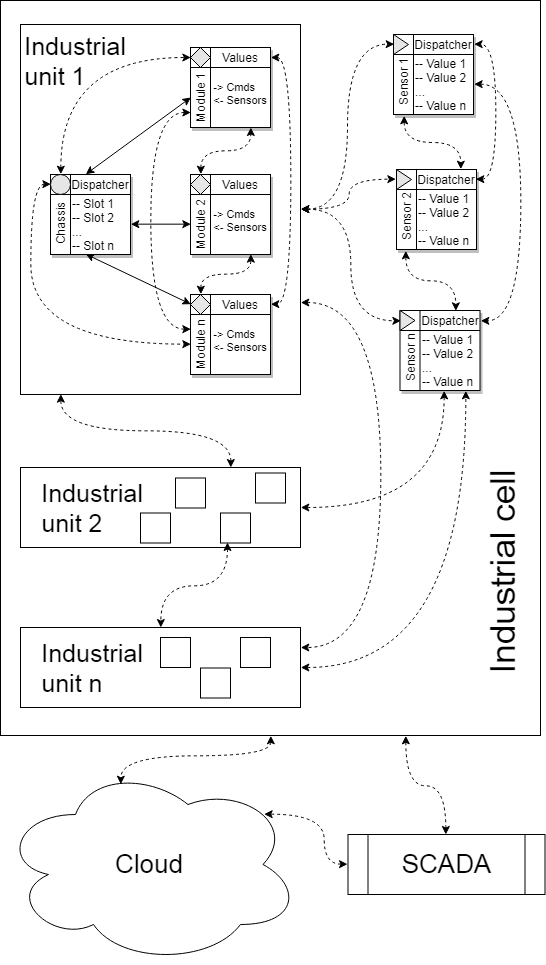
\includegraphics[width=0.5\textwidth]{ch-3/main-arch}
	}
	\caption{Слотовая модель модульного оборудования.}\label{fig:main-arch}
\end{figure}

Слот ""--- это запись типа <<ключ-значение>>, из которой диспетчер извлекает необходимые данные. Слот включает в себя следующие поля:

\begin{enumerate}
	\item адрес;
	\item название модуля/датчика;
	\item функции;
	\item возвращаемое значение;
	\item пределы возвращаемого значения.
\end{enumerate}

В качестве адреса выступают IPv6-адрес и порт, необходимые для взаимодействия с модулем. Название должно быть представлено в строковом виде или числовым идентификатором. Доступные для выполнения функции описываются набором G-кодов и М-функций в соответствии со стандартами ISO 6983-1 и ISO/TR 6983-2.
Например, фрезерная головка будет представлять возможность работать с командами M3 и M4 (запуск шпинделя по и против часовой стрелки CW/CCW), M5 (останов шпинделя) и S (скорость вращения); для лазерной головки ""--- это будут команды M3 (включить лазер), М5 (выключить) и S (задать мощность в процентах); для магазина инструментов ""--- M6 (сменить инструмент) и T (выбрать инструмент из магазина по номеру).  При этом все команды, связанные с перемещением головки в трех основных координатах определяются модулем координатного шасси.

\begin{figure}[ht]
\centerfloat{
	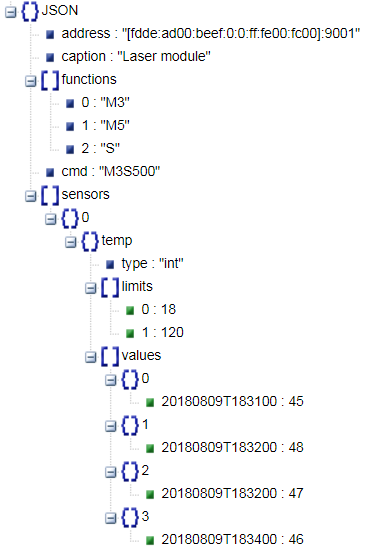
\includegraphics[width=0.3\textwidth]{ch-3/json}
}
\caption{Иерархическая структура единого реестра в формате JSON.}\label{fig:json}
\end{figure}

Возвращаемое значение не обязательно должно быть одним. Описание каждого из них включает в себя тип, пределы и массив значений с временными метками. Диспетчер контролирует выход каждого значения за допустимые пределы, и в случае возникновения такой ситуации – осуществляет анализ возникшей ошибки, и принимается решение о возможности или невозможности продолжения работы оборудования.

Рассмотрим теперь процедуру регистрации модуля в реестре диспетчера. С точки зрения протокола ""--- здесь нет никаких проблем: просто передача бинарного JSON-сообщения через очередь сообщений с последующей записью в распределенное хранилище [ссылка]. Однако не стоит забывать, что все диспетчеры и все модули находятся в единой самоорганизующейся mesh-сети. Возникает вопрос ""--- как модуль определит к какому конкретно диспетчеру он подключен физически.

Предлагается следующее решение. Физическое подключение каждого модуля реализуется по трехпроводному интерфейсу, где по двум проводникам передается питающее напряжении, а третий используется в качестве линии безопасности (safety line). Линия безопасности объединяет все модули одной единицы оборудования по схеме монтажное И. В данной схеме линия безопасности подтянута резистором к плюсу питания. Так как сопротивление между линией и землей бесконечность, а между питанием и линией равно номиналу резистора, то напряжение на линии равно напряжению питания. То есть высокий уровень или логическая единица. Как уже было сказано выше, все модули подключены к линии и могут замыкать её на землю. Соответственно, на линии будет высокий уровень тогда и только тогда, когда все модули выставят высокий уровень на своих выходах. Как только любой из модулей соединит линию с землей, на ней установится низкий логический уровень и не один модуль не сможет на это повлиять.

\begin{figure}[ht]
\centerfloat{
	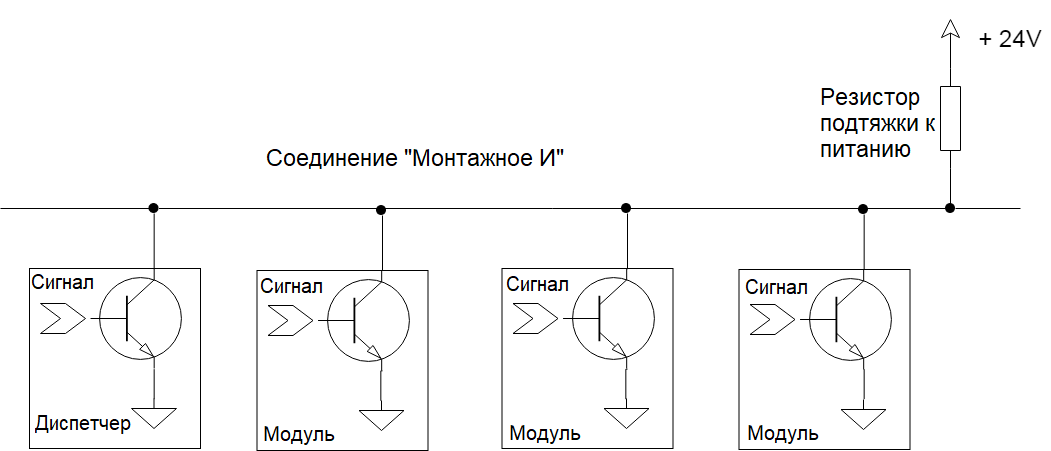
\includegraphics[width=0.7\textwidth]{ch-3/logic-and}
}
\caption{Схема шины безопасности.}\label{fig:logic-and}
\end{figure}

Таким образом, основная задача линии безопасности ""--- регистрировать аварийные ситуации. В случае возникновения аварии в любом из модулей, он просто соединяет линию безопасности с землей, что является сигналом для других модулей прекратить работу и перейти в режим восстановления после сбоя. Необходимо отметить, что к этой же линии подключена являющаяся обязательной для любого промышленного оборудования кнопка аварийного останова, а также все двери безопасности, если они предусмотрены конструкцией.

Однако в процессе инициализации модулей линия безопасности может быть использована для регистрации новых модулей. Вновь подключенный модуль вначале осуществляет подключение к сети OpenThread, затем переводит линию безопасности на низкий логический уровень. Диспетчер детектирует это, после чего получает список всех ближайших к нему узлов (neighbors в терминологии OpenThread), выбирает среди них те, которые имеют статус не подключен, после чего просит первого из них перевести линию обратно на высокий логический уровень. Если уровень изменился, значит диспетчер и модуль подключены к одной линии, следовательно, модуль может быть зарегистрирован в реестре. В противном случае, диспетчер переходит к следующему модулю в списке.

При этом нам известно, что все диспетчеры могут общаться между собой, поэтому необходимо установить правило, которое регламентирует порядок инициализации диспетчеров, то есть если один из них проводит наполнение слотов своего реестра, другие должны находится в режиме ожидания и не принимать подключения от модулей. Также понятно, что процесс подключения нового модуля может быть осуществлен только, когда оборудование находится в режиме ожидания.

\subsection{Методика определения максимальной пропускной способности канала передачи данных}

\subsection{Методика оценка качества сигнала при беспроводном соединении модулей}

В данном разделе будет рассмотрена методика оценки качество соединения при использовании модулей беспроводной связи, в частности оценено влияние факторов производственной среды, которые могут привести к ухудшению связи и способов их устранения. В производстве существует множество факторов, которые могут повлиять на помехозащищенность беспроводного сигнала. Поэтому проводятся различные исследования влияния производственной среды на беспроводной сигнал и определяются критерии его оценки. Например, шведские исследователи оценили влияние электромагнитного шума в цехах для различных диапазонов частот беспроводного сигнала~\cite{6525614, 5475862}. В ходе исследования они определили профиль снижения мощности в различных производственных помещениях с разными уровнями отражения и поглощения сигнала. Аналогичные исследования проводились также в Пекинском университете Цзяотун~\cite{Li2019}, где анализировались амплитудно-временные характеристики электромагнитных шумов на частотах 315, 433 и 916\,МГц, возникающих во время сварочных работ.
	
Также в работе~\cite{Girs2013DesignOC} описывается установка для измерения параметров беспроводного сигнала в диапазоне~\SI{2,4}{\giga\hertz}, а также методика измерения. Используя эту установку, учёные получили зависимость между стабильностью беспроводного сигнала и временем, необходимым для передачи стандартного пакета IEEE 802.15.4. В статье~\cite{8308609} рассматривается проблема шумового загрязнения в диапазоне~\SI{2,4}{\giga\hertz} другими сетями и источниками помех. Предложена математическая модель электромагнитного шума в этом диапазоне, которую можно использовать для предварительной оценки помехозащищенности производственных помещений.

Производство обычно рассматривается как иерархическая система, состоящая из уровней, как показано на~\cref{ch-3/fig-1}. На каждом уровне есть элементы сетевой инфраструктуры, обеспечивающие как горизонтальную, так и вертикальную передачу данных.
При этом типы используемых компьютерных сетей различаются на разных уровнях. Это происходит из-за того, что в зависимости от положения в иерархической системе выдвигаются различные требования к скорости передачи данных, безопасности, ширине канала, топологии, надежности и энергоэффективности. Более того, различные компьютерные сети могут сосуществовать на одном уровне в зависимости от выполняемых задач. Поэтому сетевая инфраструктура предприятия является гибридной.

\begin{figure*} [tb]
	\centering
	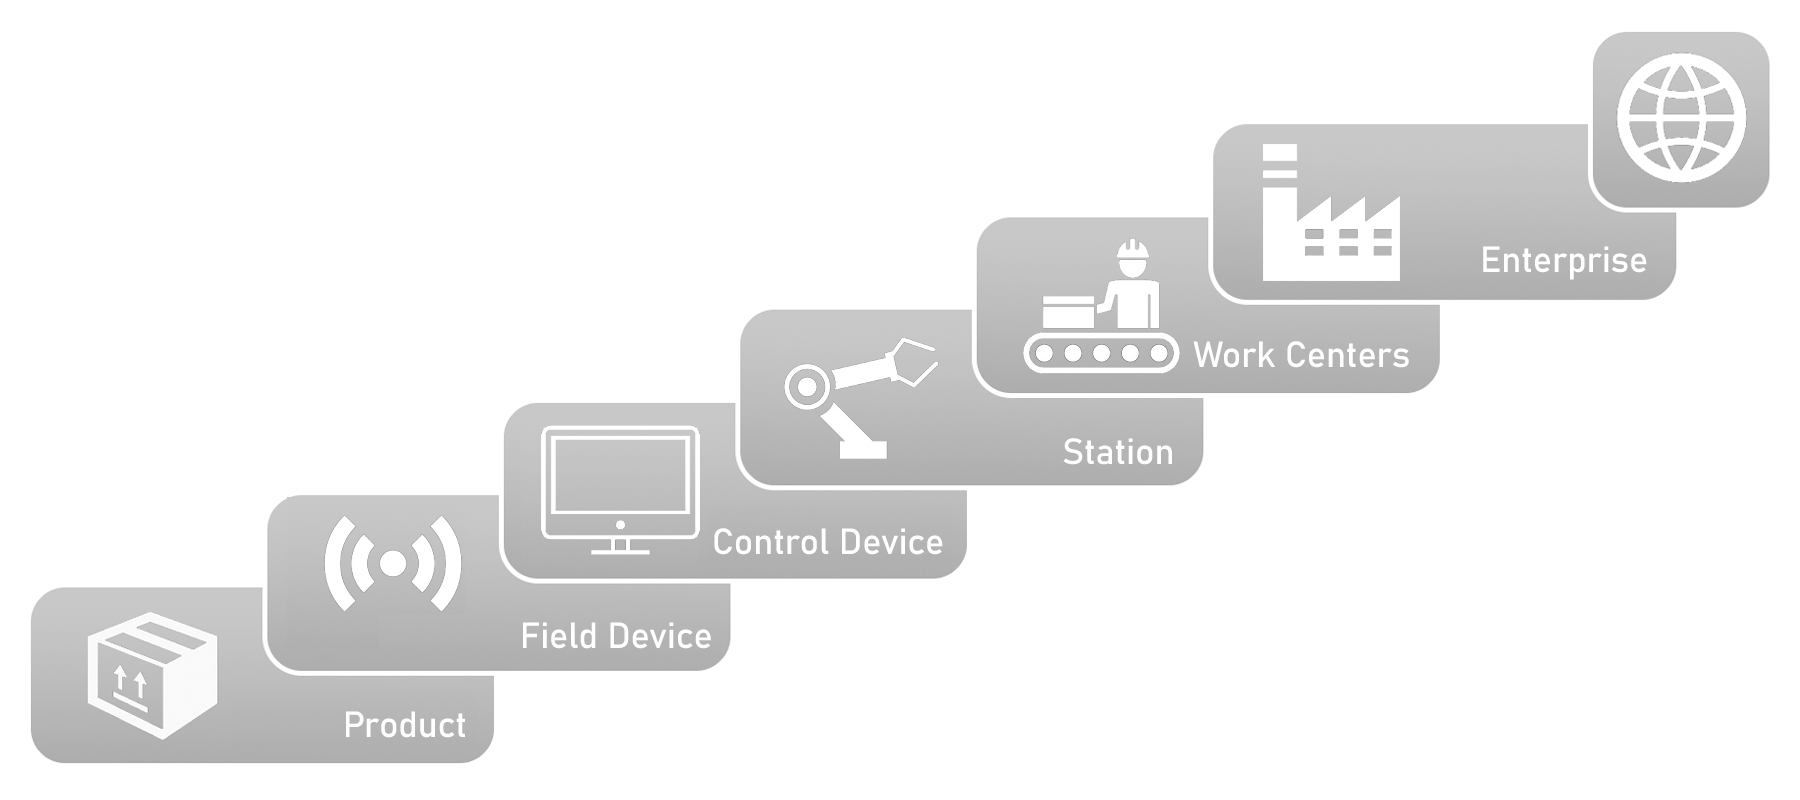
\includegraphics[width=0.9\linewidth]{ch-3/fig-1}
	\caption{Уровни производственной системы}
	\label{ch-3/fig-1}
\end{figure*}

Чтобы понять, на каких уровнях функционирует беспроводная персональная сеть, необходимо определить <<цифровых двойников>>, которые работают с данными, передаваемыми через сеть. Например, данные, полученные от станка с числовым программным управлением и/или от датчиков, установленных на нем, могут быть использованы для создания <<цифрового двойника>> этого оборудования. Кроме того, наглядным примером является ситуация, когда в цехе необходимо поддерживать определенную температуру и влажность для выполнения определенных технологических операций. В этом случае данные будут использоваться для <<цифрового двойника>> мастерской.

Беспроводные персональные вычислительные сети используются на уровнях системы управления, оборудования, производственной ячейки, цеха и, реже, в случае малых предприятий, на уровне всего предприятия. WPAN имеют широкое покрытие и применимы в производственной среде благодаря активной поддержке комитета IEEE (Институт инженеров по электротехнике и электронике). Это привело к появлению ряда технологий, охватываемых набором стандартов IEEE 802.15.4, включая хорошо известные технологии, такие как Bluetooth, ZigBee и Thread.

Одновременно стремительно растет аппаратная база. В настоящее время на рынке представлен большой выбор микросхем и готовых плат, поддерживающих сразу несколько технологий WPAN. Несмотря на изначально небольшую дальность передачи сигнала, использование сетки топология позволяет достичь практически неограниченного диапазона. Также стоит отметить возможность построения WPAN со стеком TCP/IP, что удобно при работе с другими сетями.

К недостаткам WPAN можно отнести частотные диапазоны, в которых работают эти сети: \SI{868}{\mega\hertz}, \SI{915}{\mega\hertz} и \SI{2,4}{\giga\hertz}. В России они не лицензированы, но имеют ограничения по мощности передатчика~\cite{freq}. Эти диапазоны называются <<частотами ISM>>\footnote{Сокр. от англ. \textit{Industrial, Scientific, Medical}.}. Как следует из названия, большое количество оборудования работает в диапазонах, которые могут создавать помехи сети~\cite{750064, 6209430}.

На производственной площадке существует множество факторов, которые могут ослабить и исказить беспроводной сигнал. Выявление этих аспектов перед развертыванием беспроводной сети является обязательной процедурой. Рисунок~\cref{ch-3/fig-2} представляет классификацию факторов по основным характеристикам. При проектировании нового предприятия многие из этих факторов можно определить уже на этапе разработки компоновки оборудования и агрегатов. Например, тип среды может определяться функциональным назначением производственного помещения. Зная окончательную компоновку блоков, можно определить, где офисные сети Wi-Fi~2,4\,ГГц будут пересекаться с промышленной беспроводной сетью. Учитывая это, можно вносить коррективы, чтобы повысить помехозащищенность сети.

\begin{figure*}[ht]
	\centering
	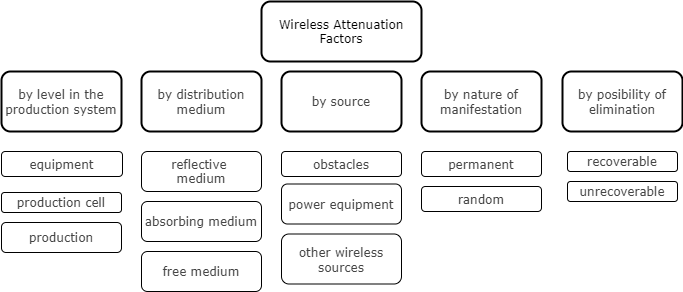
\includegraphics[width=\linewidth]{ch-3/fig-2}
	\caption{Классификация факторов ослабления беспроводного сигнала на производственной площадке}
	\label{ch-3/fig-2}
\end{figure*}

Однако внедрение беспроводной сети на уже действующей производственной площадке в настоящее время является более актуальной задачей. Кроме того, для получения достаточно точной картины измерения следует проводить непосредственно на предприятии. Для определения качества сигнала используются различные характеристики. Они включают профиль ослабления мощности, амплитудные и временные характеристики, отношение сигнал/шум~\cite{6133782} и т.\,д. К сожалению, значений этих параметров требует использования дорогостоящих инструментов "--- анализатора спектра, вектора анализатор цепей и специальные антенны. А квалификационные требования к человеку, производящему измерения, очень высоки.

В предлагаемой методике используется индикатор уровня принимаемого сигнала (RSSI). Его главное преимущество "--- встроенная поддержка практически на любом сетевом оборудовании, включая аппаратную платформу, используемую в эксперименте. Это означает, что можно получить значение RSSI от приемника без использования дополнительного измерительного оборудования. Однако RSSI нельзя использовать напрямую для измерения качества беспроводного сигнала, поскольку этот параметр может содержать значительный компонент помех. Таким образом, сильные помехи могут привести к потере пакетов при увеличении значения RSSI~\cite{8211460}.

Одновременно рассчитывается параметр $RSSI_T$, основанный на характеристиках антенн приемника и передатчика, а также с учётом частоты беспроводного сигнала и опорного параметра затухания~\cref{eq-1, eq-2, eq-3}:

\begin{equation}
	RSSI_T = A-10 \mu \log (d),
	\label{eq-1}
\end{equation}

\noindent где $d$ "--- расстояние от источника, м; $\mu$ "--- показатель ослабления, $\mu = 2$;

\begin{equation}
	A = P_{out} + G_{tx} + G_{rx} -FSPL,
	\label{eq-2}
\end{equation}

\noindent где $P_{out}$ "--- выходная мощность передатчика, дБм; $G_{tx}$ "--- усиление исходной антенны, дБи; $G_{rx}$ "--- усиление антенны приемника, дБи; $FSPL$ "--- потери на трассе в свободном пространстве, дБ;

\begin{equation}
	FSPL = 10 \log (d) +20 \log (f) +20 \log (4 \pi/c),
	\label{eq-3}
\end{equation}

\noindent где $f$ "--- частота, Гц; $c = 299792458$ м/с.

Поэтому в предлагаемом методе используется отклонение $\Delta RSSI$, полученное как разница между измеренным значением $RSSI_P$ и теоретическим значением $RSSI_T$~ \cref{eq-4}.

\begin{equation}
	\Delta RSSI = RSSI_T-RSSI_P
	\label{eq-4}
\end{equation}

Тем не менее, при проектировании сети, особенно в случае применения ячеистой топологии, сначала определяется расположение узлов в помещении. Следовательно, можно перейти от отклонения $\Delta RSSI$ к максимальному расстоянию между узлами~$D_{max}$~\cref{eq-5}, более удобному параметру для рассматриваемой задачи. Сигнал со значением RSSI менее~-80\,дБм считается слабым~\cite{mob_sig}. На основе этого утверждения и~\cref{eq-4} можно рассчитать$RSSI_T$~\cref{eq-6} на определенном расстоянии от передатчика с учетом среднего отклонения$\Delta RSSI$, на который влияют факторы конкретной производственной среды~\cref{eq-7}.

\begin{equation}
	D_{max} = 10^\frac{A-RSSI_T}{10 \mu}
	\label{eq-5}
\end{equation}

\begin{equation}
	RSSI_T = -80-\overline{{\mathit \Delta} RSSI}
	\label{eq-6}
\end{equation}

\begin{equation}
	\overline{{\mathit \Delta} RSSI} = \frac1n \sum_{\substack{0 < i < n}}{\mathit\Delta} RSSI_i,
	\label{eq-7}
\end{equation}

\noindent где $n$ "--- количество измерений. В этом случае $n = 25$.

\paragraph{План эксперимента}

Эксперимент проводился для определения существенных факторов, ослабляющих беспроводной сигнал в производственной среде. Для этого необходимо было собрать набор экспериментальных данных и оценить помехозащищенность WPAN под влиянием заданных факторов в соответствии с разработанной методикой.
Измерения были получены с использованием экспериментальной установки, показанной на~\cref{ch-3/fig-3}.

\begin{figure} [ht]
	\centering
	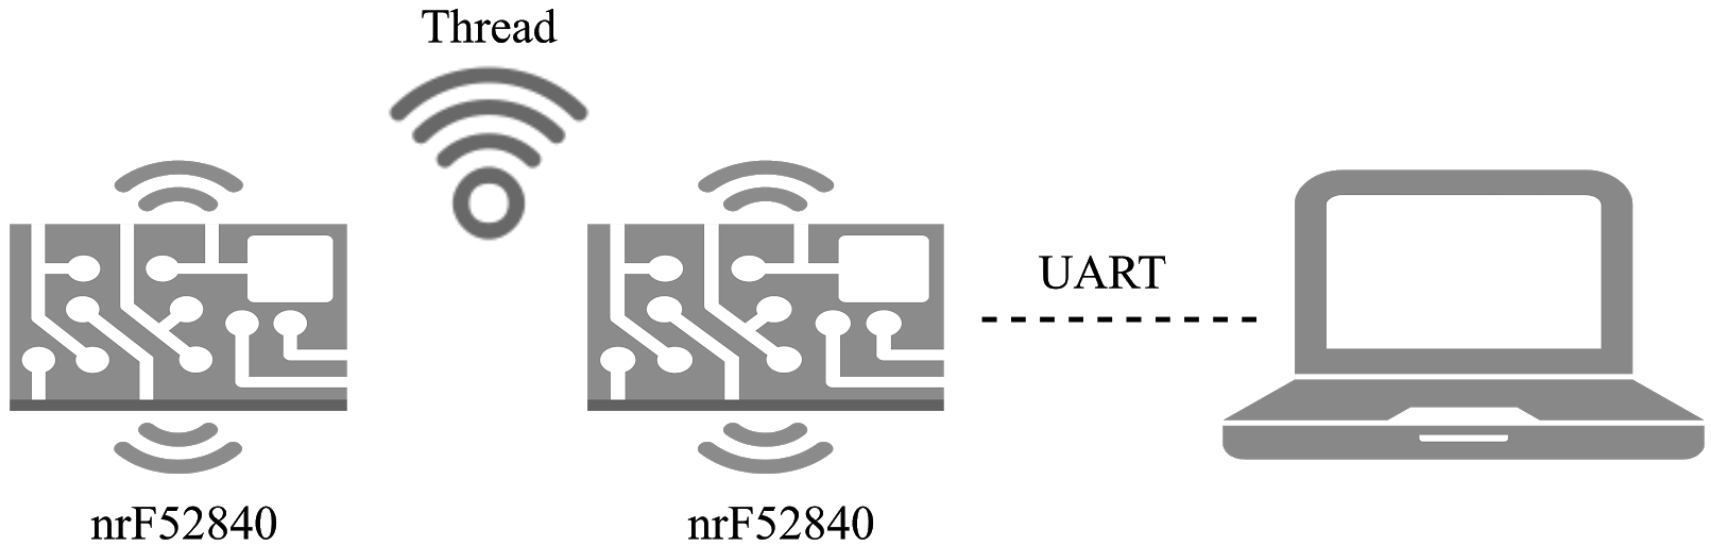
\includegraphics[width=\linewidth]{ch-3/fig-3}
	\caption{Экспериментальная установка}
	\label{ch-3/fig-3}
\end{figure}

Установка состоит из двух плат на базе микросхемы nRF52840~\footnote{Электронный ресурс: {\tiny\url{https://wiki.makerdiary.com/nrf52840-mdk-usb-dongle/} (дата обращения: 16.07.2020)}.}, которые действуют как приемник и передатчик. На плате установлена чип-антенны, параметры которой указаны в таблице~\cref{tab-1}. Кроме того, для регистрации данных используется персональный компьютер. Персональный компьютер подключен к приемнику через интерфейс универсального асинхронного приемника-передатчика (UART) для получения измеренных значений RSSI. Внутри WPAN сообщение передается по протоколу Thread~\footnote{Электронный ресурс: {\tiny\url{https://openthread.io}} (дата обращения: 20.05.2020).}.

\begin{table}[ht]
\centering
\caption{Спецификация чип-антенны ACA-2012-A1-CC-S} \vspace{4pt}
\label{tab-1}
	\begin{tabularx}{\linewidth}{XX}
		\toprule
		\textbf{Параметр} & \textbf{Значение} \\
		\midrule
		Диапазон частот (МГц) & 2400--2483 \\
		Коэффициент стоячей волны &$<3,0$\\
		Поляризация & линейная \\
		Входное сопротивление (Ом) & 50 \\
		Коэффициент усиления (дБи) & 1,72 \\
		Размеры (мм) & $2,0 \times1,2 \times0,55$\\
		\bottomrule
	\end{tabularx}
\end{table}

Эксперимент проводился на производственных площадях компании <<Лар Технологии>>, специализирующейся на разработке технологического оборудования. Влияние каждого из следующих факторов разного типа, выбранных в соответствии с классификацией в~\cref{ch-3/fig-2}, изучалось отдельно.

\begin{itemize}
\item склад металлопроката как фактор отражающей среды;
\item силовое оборудование:
	\begin{itemize}
		\item асинхронный двигатель;
		\item шаговый двигатель;
		\item сварочный аппарат;
	\end{itemize}
\item толстостенная стальная труба (толщина стенки~\SI{20}{\milli\meter}) как фактор препятствия;
\item сети (сети Wi-Fi и ZigBee).
\end{itemize}

Значения RSSI под воздействием сетей~\SI{2,4}{\giga\hertz} были зафиксированы в многоквартирном доме, так как их не было в производственных помещениях. Также были получены измерения на открытом воздухе без влияния перечисленных факторов. Эксперимент проводился в диапазоне от 0,5 до \SI{24,5}{\meter} с шагом \SI{1}{\meter}. На каждом шаге выполнялась серия измерений в течение одной минуты с периодом~\SI{1}{\second}.

\paragraph{Результаты экспериментов}

По мере увеличения расстояния между приемником и передатчиком значение RSSI уменьшается, что можно объяснить явлением потерь на трассе распространения. В этом случае значение RSSI уменьшается логарифмически в зависимости от расстояния~\cref{eq-1}. Это происходит в соответствии с законом сохранения энергии. Поскольку волна передает энергию и распространяется сферически, энергия с увеличением расстояния распределяется по увеличивающейся площади поверхности сферы~\footnote{Электронный ресурс: {\tiny\url{http://asupro.com/gps-gsm/means-identification/automatic/linear-circular-polarization-rfid-system.html}} (дата обращения: 09.05.2020).}. \cref{ch-3/fig-4a} показывает график, отражающий теоретическую кривую значений RSSI, полученных в соответствии с~\cref{eq-1}, и зависимость между RSSI и расстоянием при измерениях на открытом воздухе. Можно отметить, что кривые оказались похожими по форме. Однако есть небольшие отклонения RSSI, значения которых показаны в~\cref{ch-3/fig-4b}.

\begin{figure}[!htb]
	\centering
	\subfloat []{%
		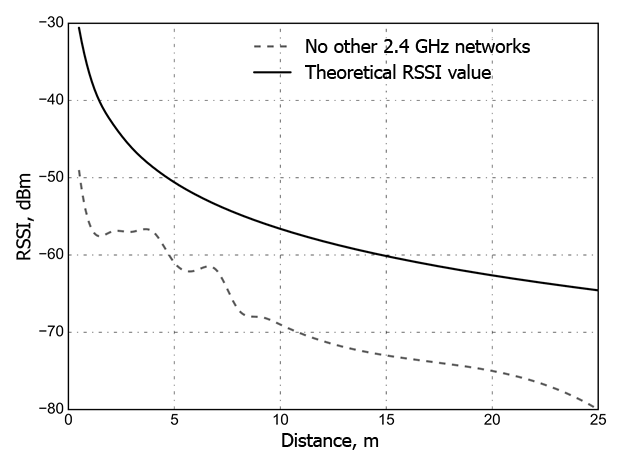
\includegraphics[clip, width=0.49\textwidth]{ch-3/fig-4a}%
		\label{ch-3/fig-4a}
	}
	\subfloat []{%
		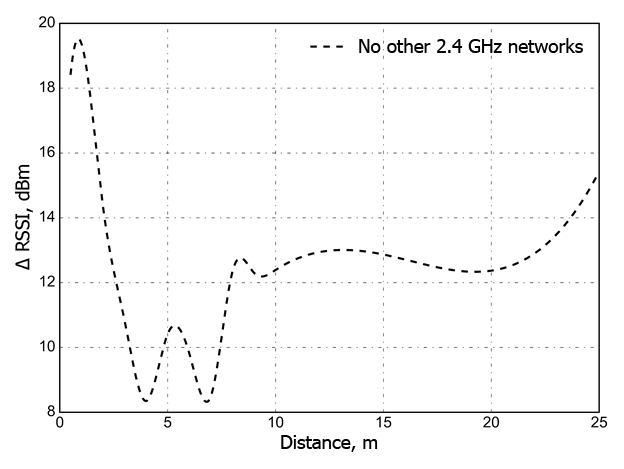
\includegraphics[clip, width=0.49\textwidth]{ch-3/fig-4b}%
		\label{ch-3/fig-4b}
	}
	\caption[Влияние характеристик приемника и передатчика на RSSI и отклонение $RSSI$ от теоретического значения]{Влияние характеристик приемника и передатчика на: $RSSI$ (\textit{а}) и отклонение $RSSI$ от теоретического значения (\textit{б})}
\end{figure}

Одной из отличительных характеристик промышленного производства является тип среды, по которой распространяется беспроводной сигнал. Производство чаще всего характеризуется отражающей средой, за некоторыми исключениями, например, целлюлозно-бумажные и деревообрабатывающие предприятия, где преобладает поглощающая среда. Распространение сигнала в отражающей среде подвержено эффекту многолучевого распространения~\cite{7433518}. В результате принимаются не только прямые, но и отраженные лучи, что приводит к колебаниям амплитуды, фазы и угла входного сигнала. На рисунке~\cref{ch-3/fig-5} показаны графики $RSSI$ и $\Delta RSSI$ в зависимости от расстояния соответственно. Графики показывают значительные колебания, вызванные указанным выше эффектом.

\begin{figure} [tb]
	\subfloat []{%
		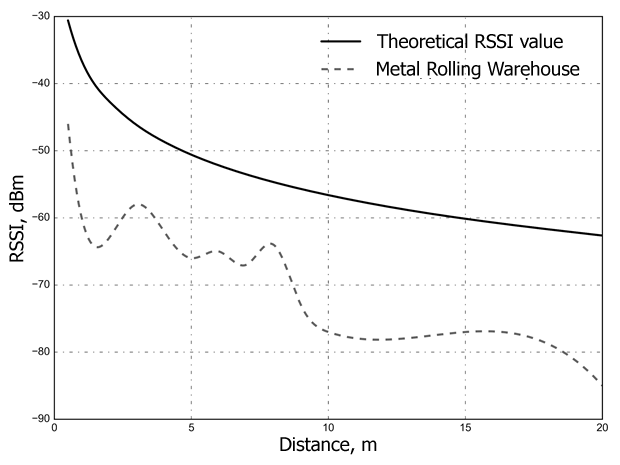
\includegraphics[clip, width=0.49\textwidth]{ch-3/fig-5a}%
		\label{ch-3/fig-5a}
	}
	\subfloat []{%
		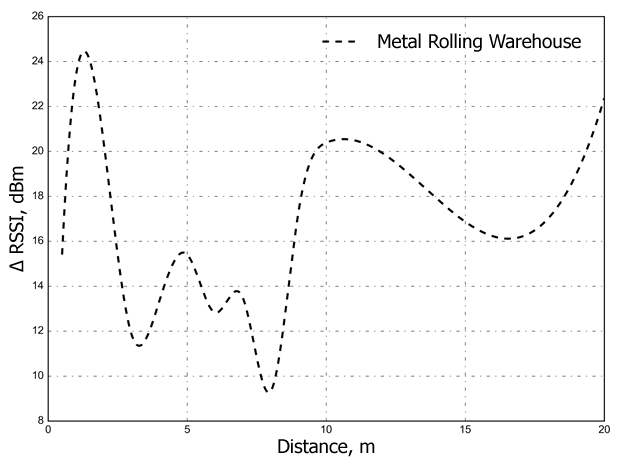
\includegraphics[clip, width=0.49\textwidth]{ch-3/fig-5b}%
		\label{ch-3/fig-5b}
	}
	\caption{Влияние отражающей среды на: $RSSI$(\textit{а}) и отклонение $RSSI$ от теоретического значения (\textit{б})}
	\label{ch-3/fig-5}
\end{figure}

Препятствия, встречающиеся на пути распространения сигнала, имеют аналогичный эффект. Кроме того, могут возникать явления дифракции (на поверхностях с резкими неровностями) и рассеяния (на шероховатых поверхностях). Стены между цехами и производственными ячейками могут отражать сигнал из-за наличия арматуры и, с другой стороны, поглощать его из-за звукоизоляции. Более того, в производственных помещениях бывают ситуации, когда приемник или передатчик может располагаться только за определенным препятствием или внутри бокса. \cref{ch-3/fig-6} показывает данные для этого случая. Полученный результат аналогичен показанному на~\cref{ch-3/fig-5}; однако отклонение $RSSI$ больше, поскольку препятствие окружало приемник и находилось в непосредственной близости от него.

\begin{figure} [tb]
	\subfloat []{%
		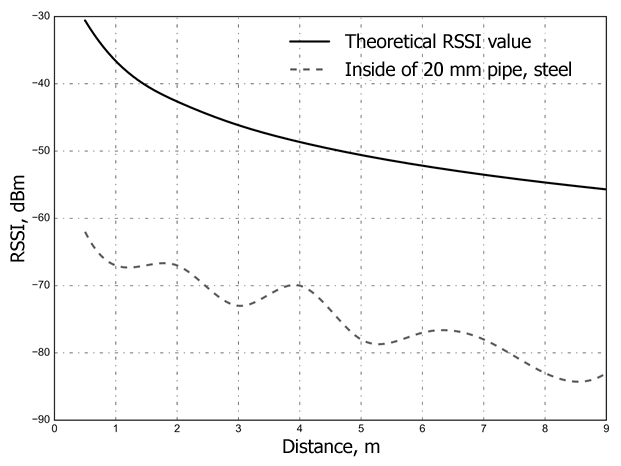
\includegraphics[clip, width=0.49\textwidth]{ch-3/fig-6a}%
		\label{ch-3/fig-6a}
	}
	\subfloat []{%
		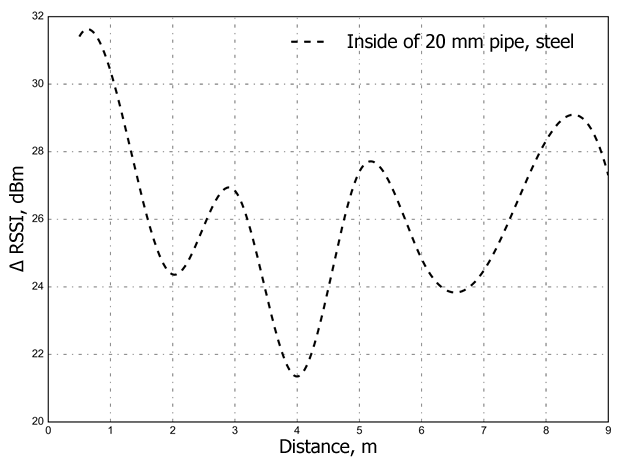
\includegraphics[clip, width=0.49\textwidth]{ch-3/fig-6b}%
		\label{ch-3/fig-6b}
	}
	\caption{Влияние препятствий в производственном помещении на: $RSSI$(\textit{а}) и отклонение RSSI от теоретического значения (\textit{б})}
	\label{ch-3/fig-6}
\end{figure}

Поскольку инфраструктура производственной сети отличается неоднородностью, вполне вероятно, что несколько беспроводных сетей будут работать одновременно в одном и том же диапазоне частот. В этом случае могут возникать интерференции, накладываются когерентные волны, что приводит к увеличению или уменьшению результирующей амплитуды. Этот эффект может быть особенно заметен, когда устройства работают на одном канале, что типично для диапазона~\SI{2,4}{\giga \hertz}, где сети Wi-Fi, Bluetooth, ZigBee и Thread пересекаются~\cite{016461}. Полученные графики в~\cref{ch-3/fig-7} показывают значительное влияние этого фактора.

\begin{figure} [htb]
	\subfloat []{%
	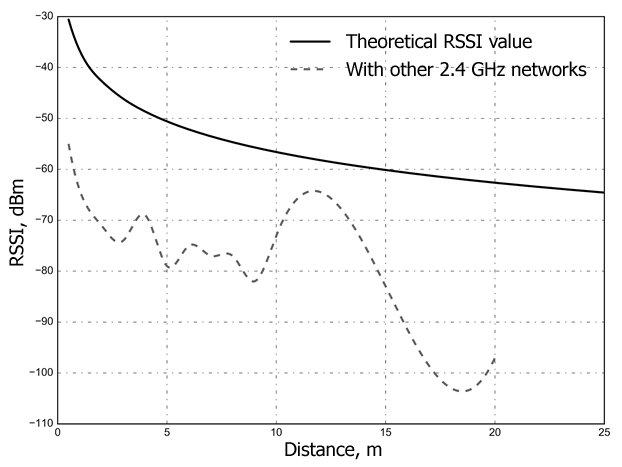
\includegraphics[clip, width=0.49\textwidth]{ch-3/fig-7a}%
	\label{ch-3/fig-7a}
	}
	\subfloat []{%
	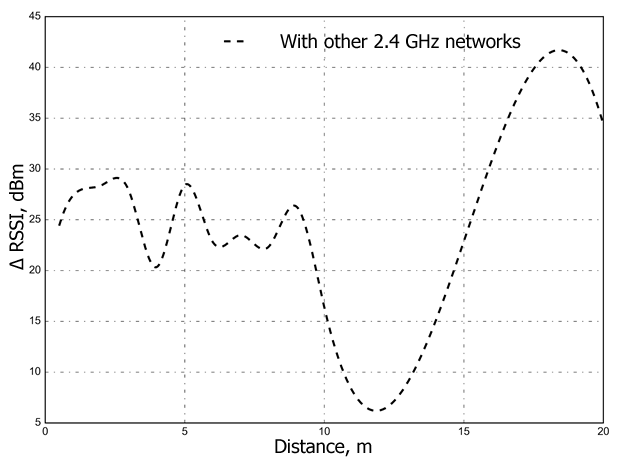
\includegraphics[clip, width=0.49\textwidth]{ch-3/fig-7b}%
	\label{ch-3/fig-7b}
	}
	\caption{Влияние соседних сетей~\SI{2,4}{\giga \hertz} на: отклонение RSSI (\textit{а}) и $RSSI$ от теоретического значения (\textit{б})}
	\label{ch-3/fig-7}
\end{figure}

Большое количество силового оборудования, расположенного в помещении мастерской, может искажать передаваемый беспроводной сигнал и вызывать помехи. Чаще всего это наблюдается при распространении импульсного сигнала по линиям электропередачи оборудования. Это происходит потому, что при формировании фронта амплитуда сигнала изменяется с большой скоростью, что приводит к появлению большого количества высокочастотных гармоник в спектре сигнала. В случае рассматриваемого в эксперименте шагового двигателя управление осуществляется с помощью широтно-импульсной модуляции (ШИМ). Графики на рисункек~\cref{ch-3/fig-8} показывают искажение беспроводного сигнала. Для асинхронного двигателя (рисунок~\cref{ch-3/fig-9}) сильных колебаний не наблюдалось, так как управление производилось без использования преобразователя частоты. Сварщик TIG показал один из худших показателей (рисунокк~\cref{ch-3/fig-10}), так как при переключении транзисторных ключей инвертора в процессе сварки на фронтах импульсов происходит большое количество кратковременных переходных процессов в виде затухающих высокочастотных колебания~\footnote{Электронный ресурс: {\tiny\url{https://303421.selcdn.ru/soel-upload/clouds/1/iblock/e03/e036d5c6f8c271c7ebbf44799619f068/201002052.pdf}} (дата обращения 01.05.2020).}.

\begin{figure} [htb]
	\subfloat []{%
	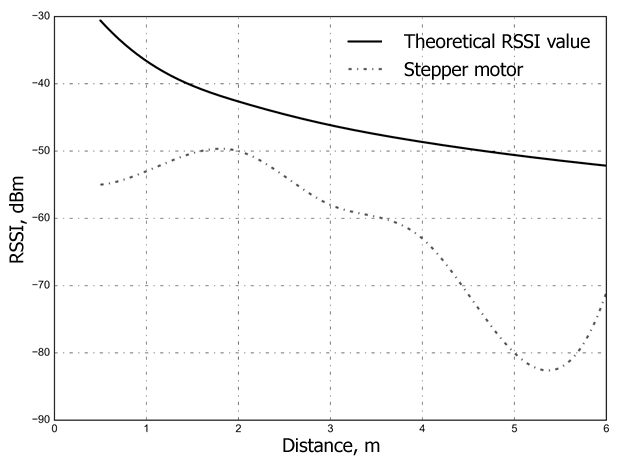
\includegraphics[clip, width=0.49\textwidth]{ch-3/fig-8a}%
	\label{ch-3/fig-8a}
	}
	\subfloat []{%
	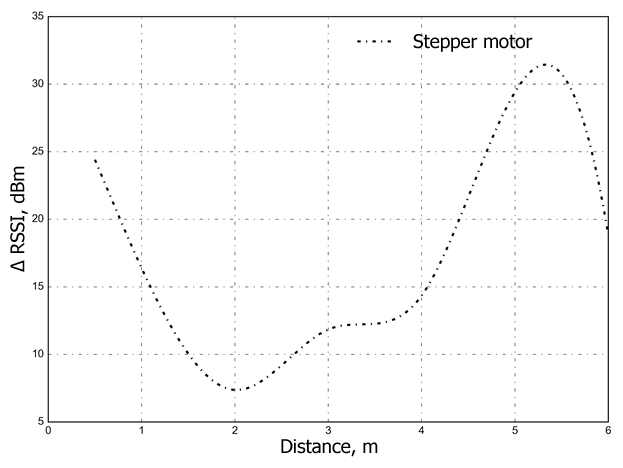
\includegraphics[clip, width=0.49\textwidth]{ch-3/fig-8b}%
	\label{ch-3/fig-8b}
	}
	\caption{Влияние исправного шагового двигателя на: отклонение $RSSI$ (\textit{а}) и $RSSI$ от теоретического значения (\textit{б})}
	\label{ch-3/fig-8}
\end{figure}

\begin{figure} [htb]
	\subfloat []{%
	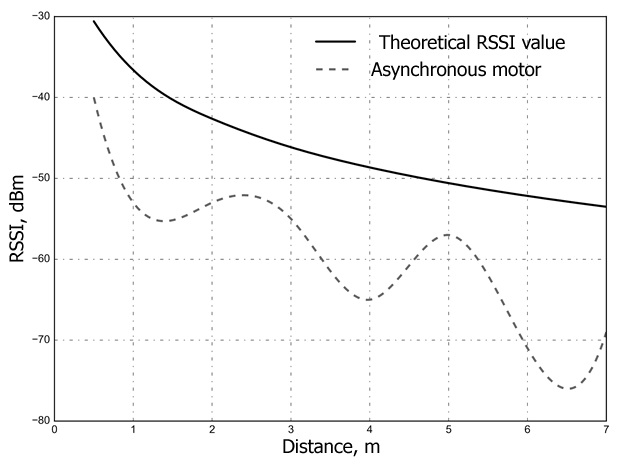
\includegraphics[clip, width=0.49\textwidth]{ch-3/fig-9a}%
	\label{ch-3/fig-9a}
	}
	\subfloat []{%
	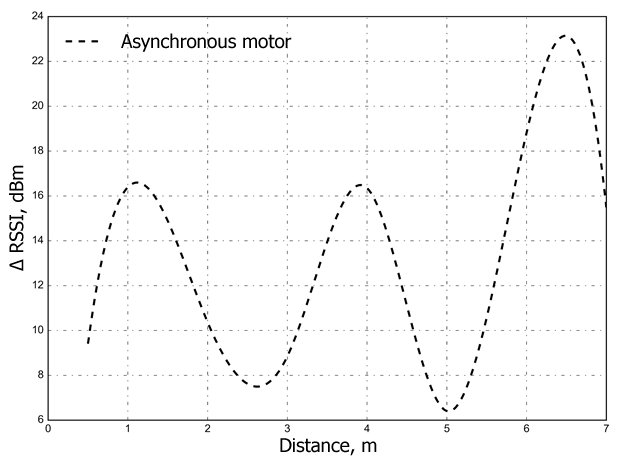
\includegraphics[clip, width=0.49\textwidth]{ch-3/fig-9b}%
	\label{ch-3/fig-9b}
	}
	\caption{Влияние работающего асинхронного двигателя на: отклонение $RSSI$ (\textit{а}) и $RSSI$ от теоретического значения (\textit{б})}
	\label{ch-3/fig-9}
\end{figure}

\begin{figure} [htb]
	\subfloat []{%
	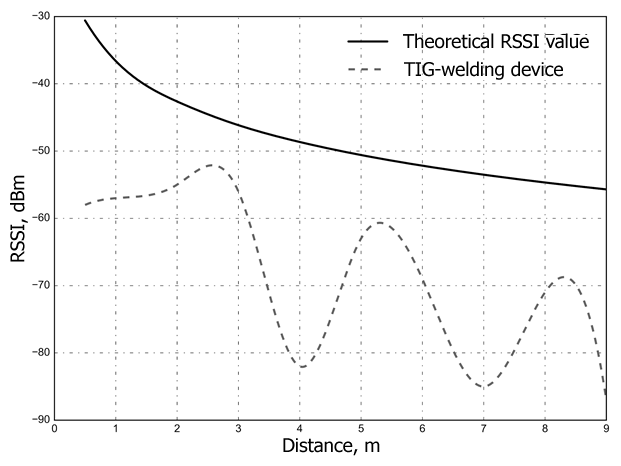
\includegraphics[clip, width=0.49\textwidth]{ch-3/fig-10a}%
	\label{ch-3/fig-10a}
	}
	\subfloat []{%
	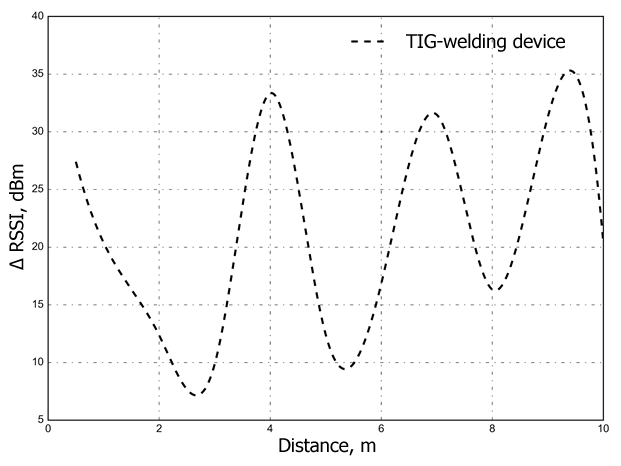
\includegraphics[clip, width=0.49\textwidth]{ch-3/fig-10b}%
	\label{ch-3/fig-10b}
	}
	\caption{Влияние работающего сварочного аппарата TIG на: отклонение $RSSI$ (\textit{а}) и $RSSI$ от теоретического значения (\textit{б})}
	\label{ch-3/fig-10}
\end{figure}

В таблице~\cref{tab-2} приводятся результаты серии экспериментов. Наихудший результат был получен в эксперименте, когда ствольная коробка была помещена в толстостенную стальную трубу. Это означает, что этого приемника следует избегать или его следует располагать не дальше~6,85\,м от передатчика. Наилучшие результаты были показаны при измерении RSSI в свободной среде.

Имеется небольшое отклонение от теоретического значения. Из-за некоторых аппаратных особенностей антенны, которые не учитывались в расчетах, и среднего теоретического значения показателя затухания. Следует отметить, что возможность организации WPAN на основе топологии ячеистой сети позволяет нейтрализовать негативные эффекты за счет плотного расположения сетевых узлов, согласно рассчитанному~$D_{max}$.

\begin{table} [!ht]
\centering
\caption{Влияние производственных факторов на помехозащищенность беспроводных персональных сетей (WPAN)} \vspace{4pt}
\label{tab-2}
\begin{threeparttable}
\begin{tabularx}{\linewidth}{@{} lrrr}
	\toprule
	\textbf{Факторы} &
	{\scriptsize $\Delta R$} \tnote{1} &
	{\scriptsize $\Delta R_{max}$} \tnote{2} &
	{\scriptsize $D_{max}$} \tnote{3} \\
	\midrule
	\scriptsize Бесплатная среда без других сетей \SI{2,4}{\giga\hertz} & 12,37 & 18,82 & 34,22 \\
	\scriptsize Асинхронный двигатель & 12.69 & 19.37 & 33.99 \\
	\scriptsize Отражающая среда (склад металла) & 16.33 & 23.39 & 22.54 \\
	\scriptsize Шаговый двигатель & 17.51 & 29.41 & 19.67 \\
	\scriptsize сварщик TIG & 21.11 & 34.35 & 13.01 \\
	\scriptsize Medium с шумом от других сетей \SI{2,4}{\giga\hertz} & 25,03 & 32,37 & 8,27 \\
	\scriptsize Экранирование толстостенной стальной трубой & 26,67 & 34,41 & 6,85 \\
	\bottomrule
\end{tabularx}
\begin{tablenotes} \footnotesize
	\item [1] Средняя ошибка $\Delta RSSI$, дБм
	\item [2] Максимальная ошибка $\Delta RSSI_{max}$, дБм
	\item [3] Максимальное расстояние между передатчиками, м
\end{tablenotes}
\end{threeparttable}
\end{table}

Подводя итог, в документе описывается серия экспериментов, которые определяют помехоустойчивость WPAN в производственной среде. Предлагается метод оценки помехозащищенности сетей данного типа на основе $RSSI$. Выявлены факторы ослабления беспроводного сигнала и рассчитаны значения помехоустойчивости на реальной производственной площадке.

Учитывая полученные данные, можно сделать вывод, что многие производственные факторы оказывают существенное влияние на качество сигнала WPAN. Однако воздействие недостаточно велико, чтобы избежать использования этой технологии. Более того, влияние многих факторов может быть уменьшено за счет использования топологии ячеистой сети и плотного расположения приемников и передатчиков. Стоит подчеркнуть важность проведения соответствующих измерений для каждого конкретного производства, поскольку это обеспечивает эффективное размещение приемников и передатчиков в производственных помещениях.

Результаты особенно интересны в контексте оцифровки производства, где беспроводной метод передачи данных от датчиков уровня поля становится предпочтительнее проводного из-за требований гибкости и мобильности производственного процесса.

\section{Выводы по главе 3}

\FloatBarrier